\documentclass{article}
\usepackage{graphicx}
\usepackage{graphicx} 
\usepackage{amssymb}
\usepackage{float}
\usepackage{amsmath}
\usepackage{algorithm}
\usepackage{algpseudocode}
\usepackage{indentfirst}

\title{Perceptron}
\author{ }
\date{ }

\begin{document}
	
	\maketitle 

    Perceptron is a more sophisticated learning algorithm for producing linear classifiers. 
    
    \begin{algorithm}
    \begin{algorithmic}[]
        \State \textbf{Input:} $D_n$, $T$
        \State $\theta = \overline{\theta}$
        \State $\theta_0 = 0$
        \For{$t = 1$ to $T$}
            \For{$i=1$ to $n$}
                \If{$y^{(i)}(\theta^Tx^{i}+\theta_0)\leq0$}
                    \State $\theta = \theta + y^{(i)}x^{(i)}$
                    \State $\theta_0 = \theta_0+y^{(i)}$
                \EndIf
            \EndFor    
        \EndFor \\
        \Return $\theta, \theta_0$
    \end{algorithmic}
    \end{algorithm}

    The algorithm iterates through the dataset $D_n$ $T$ times ($T$ is a hyperparameter). At each point in the dataset, it checks if $y^{(i)}(\theta^Tx^{(i)}+\theta_0)\leq0$. The if statement basically determines whether or not the current $\theta$ classified the point at index $i$ correctly. If $(x^{(i)}, y^{(i)})$ were correctly classified, then $y^{(i)}(\theta^Tx^{(i)}+\theta_0)$ would be positive. Recall that $\theta^Tx^{(i)}+\theta_0$ is the input to the sign function in the linear classifier hypothesis. Thus, if it is negative and $y^{(i)}$ is also negative, their product should be positive. If both are positive, their product is positive too. If they are of different signs (an incorrect classification occurred), then the if statement would trigger some modifications. In particular, it modifies $\theta$ to $\theta+y^{(i)}x^{(i)}$ and $\theta_0$ to $\theta_0+y^{(i)}$. \\

    The modifications that perceptron makes to the parameters $\theta$ and $\theta_0$ probably are not the obvious ``right move." One is probably left wondering why Rosenblatt, the inventor of perceptron, chose to set $\theta=\theta+y^{(i)}x^{(i)}$ and $\theta_0=\theta_0+y^{(i)}$. This brings up another interesting discussion point. Whereas the inner workings of most algorithms have been built intuitively around the problem to be solved, perceptron was simply introduced and left for scholars to analyze over the decades. Years of papers have determined that Rosenblatt's modifications are quite functional. \\

    To better analyze how perceptron works and even introduce a theorem about it, exploring a simpler version of the algorithm is useful. Think of perceptron-through-origin as perceptron without any offset ($\theta_0$) parameter. Some playing with dimensions later on will show that what applies to perceptron-through-origin applies to perceptron with an offset. 

    \section{Linear Separability}
    Linear separability is a property of a dataset $D_n$. $D_n$ is linearly separable when there exists some $\theta$ (no $\theta_0$ because the current discussion is about perceptron-through-origin) such that $y^{(i)}(\theta^Tx^{(i)})>0$ for all $i$. In other words, all points in the dataset $D_n$ are correctly classified. 

    \begin{figure}[H]
        \centering
        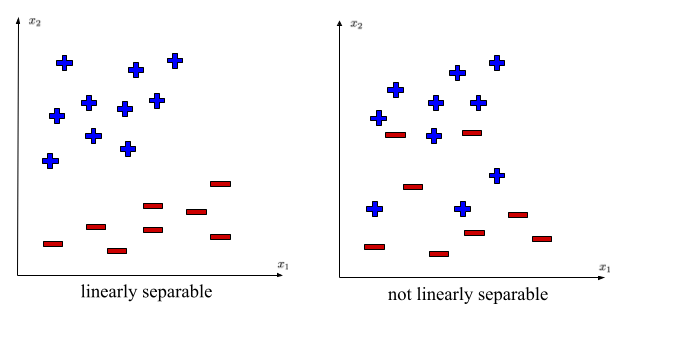
\includegraphics[width=0.5\linewidth]{Linear Separability.png}
    \end{figure}

    \section{Margin}
    The margin of a data point $(x,y)$ with repsect to a linear separator (a hyperplane) is $y{{\theta^Tx}\over{||\theta||}}$. ${\theta^Tx}\over{||\theta||}$ is the signed distance from the point to the separator. If $y$ is $-1$ and $(x,y)$ is correctly classified, then ${\theta^Tx}\over{||\theta||}$ should be negative. $y$ is the target label (either $+1$ or $-1$). Therefore, a correctly classified point should have a positive margin. An incorrectly classified point should have a negative margin. A higher margin is better because the farther a point is away from the classifier, the better classified it is (not a close call). 

    \begin{figure}[H]
        \centering
        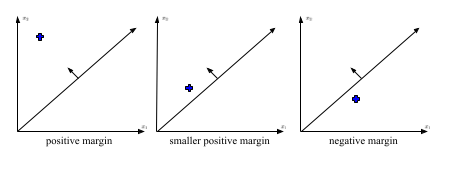
\includegraphics[width=0.5\linewidth]{Margin of a Point.png}
    \end{figure}

    The margin of an entire dataset with respect to a linear separator is equal to the margin of the point it contains that has the lowest margin: $\min_{i}{y^{(i)}{{\theta^Tx^{(i)}}\over{||\theta||}}}$.

    \section{Perceptron Convergence Theorem}
    The perceptron convergence states that if (a) there exists some $\theta^*$ such that $y^{(i)}{{\theta^Tx^{(i)}}\over{||\theta||}}>\gamma>0$ for all $i$ (in other words, if the margin of the dataset with respect to $\theta^*$) is greater than or equal to some constant $\gamma$) and (b) $||x^{(i)}||\leq{R}$ for all $i$ (in other words, when graphed, the data points are contained in a circle of radius $R$), then the perceptron will make at most $({{R}\over{\gamma}})^2$ modifications during training. 

    \section{Proof of the Perceptron Convergence Theorem}
    Say that $\theta^{(k)}$ is the hypothesis produced after $k$ modifications during training and $\theta^*$ is the parameter such that $y^{(i)}{{\theta^{*T}x^{(i)}}\over{||\theta^*||}}\geq\gamma>0$ for all $i$. The angle between $\theta^{(k)}$ and $\theta^*$ is $\alpha$. To show that $\theta^{(k)}$ will converge to become $\theta^*$ as $k$ increases, one must show that the angle $\alpha$ becomes smaller and smaller. As the angle becomes smaller, its cosine should become greater (i.e. $\cos{\alpha}$ should increase). 

    \begin{enumerate}
        \item There is a formula that describes the cosine of the angle $\alpha$ between two vectors: $\cos{\alpha}={{a\cdot{b}}\over{||a|||b||}}$. Thus, $\cos{\alpha}={{\theta^*\cdot\theta^{(k)}}\over{||\theta^*|||\theta^{(k)}||}}$. 
        \item One can break ${{\theta^*\cdot\theta^{(k)}}\over{||\theta^*||||\theta^{(k)}||}}$ down into ${{\theta^*\cdot\theta^{(k)}}\over{||\theta^*||}}\cdot{1\over{||\theta^{(k)}||}}$. 
        \item First, one should analyze ${{\theta^*\cdot\theta^{(k)}}\over{||\theta^*||}}$. $\theta^{(k)}=(\theta^{(k-1)}+y^{(i)}x^{(i)})$ when $i$ is the index of the point at which perceptron made its last modification to $\theta$. Using this information, ${{\theta^*\cdot\theta^{(k)}}\over{||\theta^*||}}={{(\theta^{(k-1)}+y^{(i)}x^{(i)})\theta^*}\over{||\theta^*||}}={{\theta^{(k-1)}\cdot\theta^*}\over{||\theta^*||}}+{{y^{(i)}x^{(i)}\cdot\theta^*}\over{||\theta^*||}}$. Recall that ${{y^{(i)}x^{(i)}\cdot\theta^*}\over{||\theta^*||}}$ is the margin, which is greater than or equal to $\gamma$. Thus, ${{\theta^{(k-1)}\cdot\theta^*}\over{||\theta^*||}}+{{y^{(i)}x^{(i)}\cdot\theta^*}\over{||\theta^*||}}\geq{k\gamma}$. 
        \item Now, one may analyze ${1}\over{||\theta^{(k)}||}$. $||\theta^{(k)}||^2 = ||\theta^{(k-1)}+y^{(i)}x^{(i)}||^2=||\theta^{(k-1)}||^2+2y^{(i)}\theta^{(k-1)}\cdot{x^{(i)}}+||x^{(i)}||^2$. It is given in the perceptron convergence theorem that $||x^{(i)}||^2 \leq R^2$. Also, $2y^{(i)}\theta^{(k-1)}\cdot{x^{(i)}}$ is negative because $\theta^{k}$ made a mistake. Therefore, $||\theta^{(k-1)}||^2+2y^{(i)}\theta^{(k-1)}\cdot{x^{(i)}}+||x^{(i)}||^2\leq{kR^2}$. Thus, ${1\over||\theta^{(k)}||}\geq{1\over{\sqrt{k}R}}$. 
        \item Putting everything together, $\cos{\alpha} \geq {\sqrt{k}}{{\gamma}\over{R}}$. Provided that cosine's greatest output is 1, $1\geq{{\sqrt{k}\gamma}\over{R}}$, so $k\leq{({{R}\over{\gamma}})^2}$. 
         
    \end{enumerate}
        
    
\end{document}



























